\section{Missing Events and the Shared Planner}
\label{app:feedbackdetails}
Section~\ref{sec:feedback} shows how pointer readings correct the belief
after missing turns. Section~\ref{sec:regimes} shows how cyclic beliefs
improve sensing decisions under a shared planner.

\subsection{Estimation and control protocol}
The four-position valve starts from a uniformly drawn position shown by an
exact initial pointer. Each step moves the valve by $-1$, $0$, or $+1$ with
nominal probabilities $(0.25,0.50,0.25)$. The missing-token schedule starts
at a random offset in each episode. The pointer reports the true state
with probability $\rho=0.8$ and otherwise draws a uniform token. The filter
uses $\ell(y\mid s)=\rho\,\mathbf{1}\{s=y\}+(1-\rho)/4$ with a learned
reliability. Both filters learn the event encoder. The GRU and phase
rotation share the filters' observation channels, encoder width, and
training budget.

Nominal Bayes uses the training parameters, and matched Bayes uses the test
parameters. Both compute the posterior from the same observation histories
as the learned models. The tests vary the run of missing turns and the period
between readings, change the turn probabilities to $(0.40,0.20,0.40)$ or
the pointer reliability to $\rho=0.6$, and include a clean case with all
turns visible and only the initial pointer.

\myparagraph{Token constraint and remaining uncertainty.} Adding the token constraint changes NLL by $-0.00095$ nats (descriptive 95\%
seed-bootstrap interval $[-0.00189,-0.00016]$) and net utility by $+0.098$ points
($[-0.048,0.246]$). The constrained filter comes within $0.0168$ nats of
matched Bayes. On the clean length-80 histories, the constraint fixes every
update and its NLL is zero, compared with $0.068$ without the constraint.
The matched posterior retains an average
entropy of $0.826$ nats for four-step bursts, compared with $0.558$ nats for
one-step bursts.

Training uses 600 Adam updates, batch size 96, gradient norm clipping at 1,
history lengths 6, 10, and 14, and dense negative log likelihood of the
latent state at each prefix. Clean episodes account for a quarter of updates.
Other episodes sample burst sizes 1 and 3 and pointer periods 6 and 9.
The validation grid consists of the clean case and all four training-regime
burst-period pairs at length 14. Using seeds 310 and 311 and disjoint
validation streams, we select the learning rate by mean final validation NLL
over the grid. The grid includes $0.001$ and $0.003$. The four learned estimators
select $0.003$. The confirmation runs use seeds 410--414 with independently
generated held-out histories. For each seed and cell there are 512 paired
episodes. We evaluate history lengths 40 and 80. The held-out nominal grid
uses periods 8 and 12 and burst sizes 1 and 4, alongside clean histories and
the two separate shifts at period 12 and burst size 4. The settings were
designed after an earlier pilot and fixed before this experiment's test results.

The input is an eight-channel vector of four event tokens and four pointer
states, with zero pointer channels if a reading is absent. Only the exact
initial pointer is supplied at step zero. No future information, final flag,
latent update counts, clock or target enters the estimator. Parameters and
optimization histories are saved for every model and seed. At test time,
all models use the same histories, targets and exogenous draws for actuation
and sensor noise.

Circular estimation actions minimize the posterior expectation of the distance
$d(a,s)=\min(|a-s|,4-|a-s|)$. Circular regret is this decision's conditional
risk minus the minimum risk, both evaluated under the matched posterior.
We also record Brier score, top-label calibration error with ten bins, KL to
the matched posterior, and NLL by observation age and latent update count.
For NLL and KL, predicted probabilities are floored at $10^{-8}$.
The seed-bootstrap intervals in the main text are descriptive percentile
intervals over 10,000 resampled sets of five paired seeds.

The planner receives a uniformly drawn target after each tracking history.
In the default setting it has at most three actions, turn success of $0.8$
without confirmation, and control-time pointer reliability $\rho=0.8$
independent of the tracking reliability. A turn costs $0.04$, a reading
costs $0.08$, and utility is reported in points on a scale of 100. The
simulator and planner are shared, so utility differences come from the
starting beliefs.

The controller computes its action values by enumerating all later actions
and every possible sensor reading. For a commanded turn by $j$ positions, the
planned belief update is $0.8 P_j b + 0.2b$. Sensing updates the belief by the pointer
likelihood and averages continuation value over possible outcomes. Greedy
selection uses these finite-horizon values at every actual decision.
We independently verify short-horizon posteriors by summing over latent
trajectories. We also verify probability normalization, finite gradients,
causality at a shared prefix and basic planner decisions.

Figure~\ref{fig:feedback} shows how pointer readings sharpen the belief and
how the resulting estimates perform under the shared planner. At length 80
under the pointer-noise shift, matched Bayes leads to $1.05$ readings per
episode and the token-constrained filter to $0.68$, for net utilities of
$59.9$ and $58.6$ points, respectively.

\begin{figure}[H]
\centering
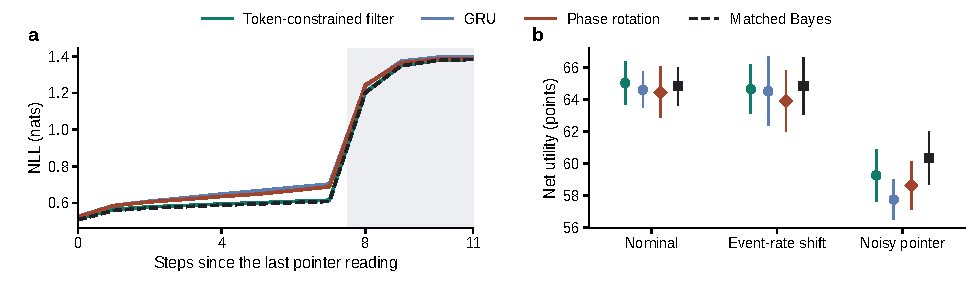
\includegraphics[width=\linewidth]{figures/feedback_results.pdf}
\caption{(a)~Nominal NLL at $L=80$ is averaged over five seeds and plotted
against steps since the last pointer reading.
Shading marks missing turns, and age zero includes the exact initial pointer
and later readings.
The dashed curve shows matched Bayes, and solid curves show the
token-constrained filter, GRU, and phase rotation.
(b)~Points show mean net utility in the nominal, event-rate shift, and
noisy-pointer regimes over $L=40,80$ and five seeds, with bars showing one
sample SD across seeds.}
\label{fig:feedback}
\end{figure}

\subsection{Planner regime sweep}
\label{app:regimes}
The sweep reuses the twenty frozen test checkpoints and the evaluation histories of the
main experiment. We vary the controller horizon $T_{\mathrm{plan}}$, the sensing
cost $c$, and the probability $\rho$ of returning the true pointer during
control. Otherwise the sensor returns a uniform token. The planner uses $\rho$
in its belief update.
Turn cost $0.04$ and turn success $0.8$ stay fixed. Action and sensor outcomes are drawn
once per cell and seed and shared by all estimators. With the original draws, $T_{\mathrm{plan}}=3$,
$c=0.08$ and $\rho=0.8$, the sweep code reproduces every per-seed utility of
Table~\ref{tab:feedback} exactly. A one-step planner never senses, and a cost of $0.4$
suppresses sensing at $\rho=0.6$, so the 75 grid points contain 53 distinct regimes.
Table~\ref{tab:regimes} shows that the cyclic filters retain the largest
minimum share of attainable utility among learned estimators.

Estimation headroom ranges from $0.3$ to $26$ points. Every learned
estimator stays within $1.5$ points of matched Bayes, and the
token-constrained filter stays within $0.66$ points. With at least ten
points of headroom, every learned estimator retains at least $89.8\%$ of
the available gain. The largest paired gain of the token-constrained
filter over the GRU is $1.47$ points.

\begin{table}[H]
\centering\small
\caption{Utility across the 75-regime planner grid. Loss to matched Bayes is
in percentage points, based on five paired seeds per regime. Retained share
uses the 40 regimes with at least ten points of headroom. Significant
losses count regimes with a seed-bootstrap interval below zero.}
\label{tab:regimes}
\begin{tabular}{lrrrrr}
\toprule
Estimator & Max loss & Mean loss & Min retained & Below uniform & Significant losses \\
\midrule
GRU & 1.47 & 0.65 & 90.1\% & 3 & 57 \\
Phase-rotation model & 1.32 & 0.63 & 89.8\% & 0 & 65 \\
Unconstrained filter & 0.66 & 0.23 & 96.6\% & 0 & 27 \\
Token-constrained filter & 0.66 & 0.21 & 95.6\% & 0 & 22 \\
Nominal Bayes & 0.73 & 0.34 & 95.4\% & 0 & 56 \\
\bottomrule
\end{tabular}
\end{table}

\FloatBarrier
